% !TeX spellcheck = en_GB

\chapter{Introduction}
\label{ch:introduction}
\lhead{Chapter \thechapter. \emph{Introduction}}

\section{Context}

\subsection{\acrfullpl{manet}}\label{manets}

With the explosive growth in the use of mobile telephony and the increasing miniaturisation and efficiency gains of portable communications devices, the classical paradigm of broadcast/receiver (or server/client) communications has given way to an increasing use of decentralised, ad-hoc networks that take advantage of this network dynamism to improve service efficiency.

Whether these networks are decentralised cellular / \gls{rf} / 802.11 WiFi networks for use in disaster relief areas~\cite{Milliken2015} or biologically inspired wireless sensor networks for low-energy, low-maintenance environmental monitoring~\cite{Nicholson2008,Selvakennedy2007}, \gls{manet} theory has gone from its first formal definition, emerging from \glspl{darpa} Packet Radio Network research, to being an integral part of modern practical communications~\cite{Jubin1987}.

Minimally, a \gls{manet} consists of of a collection of mobile physical entities (nodes) that communicate cooperatively to collect, distribute, disseminate, and collate data and/or influence across an area.
In most cases \gls{manet} nodes incorporate bi-directional transceivers to send and receive data\footnote{However this bi-directionality is not always a requirement; for example in the area of \gls{wsn}~\cite{Akyildiz2002})}
\glspl{manet} may utilise omnidirectional, static, or steerable communications antennae, and a selection of protocols such as WiFi, Bluetooth, \gls{gsm}, \gls{umts}, as well as Optical or Acoustic media, and may incorporate a range of mobilities across nodes, from static devices, terrestrial and marine surface platforms, as well as aerial and underwater platforms.
A core characteristic of \glspl{manet} is the inclusion and integration of heterogeneous node collections, i.e.\ different nodes or groups of nodes in a network may have different capabilities in terms of propulsion, sensor apparatus, communications capability, etc.

\glspl{manet} may be totally independent with no external connections, may include independent per-node communications backhauls (e.g. Cellular Modems in mobile phones as part of a Bluetooth Personal Area Network), or include static nodes that provide infrastructure based backhaul.
However, this multiplicity of variations and options presents several challenges to users and operators; the physical topology of \glspl{manet} can vary wildly over short periods of time.
A particular challenge to \gls{manet} operation is that given any node may operate as a routing / gateway node, if/when that node moves to a different region, network segments that had previously used that node as a routing path must renegotiate / re-establish their routes.
These situations, if not appropriately managed, lead to opportunities for subversion and selfishness.

The characteristics of \gls{manet}s as defined by Corson et al.\ are paraphrased in Table~\ref{tab:manet_characteristics}.

\begin{table}[h!]
  \hyphenpenalty=10000
\caption[Summary of Characteristics of \glspl{manet}]{Summary of Characteristics of \glspl{manet}~\citet{Corson1999}}
\label{tab:manet_characteristics}
  \begin{tabularx}{\textwidth}{p{2cm}X}\toprule
    Dynamic Topologies & Nodes are free to move arbitrarily; thus, the typically multi-hop network topology may change randomly and rapidly at unpredictable times, and may consist of both bidirectional and unidirectional links.
\\
    Bandwidth Constrained, Varied Capacity & Wireless links will continue to have significantly lower capacity than their hardwired counterparts.
In addition, the realized throughput of wireless communications, after accounting for the effects of multiple access, fading, noise, and interference conditions, etc., is often much less than a radio's maximum transmission rate.
\par
One effect of the relatively low to moderate link capacities is that congestion is typically the norm rather than the exception, i.e.\  aggregate application demand will likely approach or exceed network capacity frequently.\\
    Energy Constrained Operation &  Some or all of the nodes in a \gls{manet} may rely on batteries or other exhaustible means for their energy.
For these nodes, the most important system design criteria for optimization may be energy conservation.\\
    Limited physical security & Mobile wireless networks are generally more prone to physical security threats than are fixed cable nets.
The increased possibility of eavesdropping, spoofing, and denial-of-service attacks should be carefully considered.\par
Existing link security techniques are often applied within wireless networks to reduce security threats.
As a benefit, the decentralized nature of network control in \glspl{manet} provides additional robustness against the single points of failure of more centralized approaches.\\\bottomrule
\end{tabularx}
\end{table}


\subsubsection{\glspl{manet} in Harsh Environments}

As \glspl{manet} grow beyond the terrestrial arena, their operation and the protocols designed around them must be reviewed to assess their suitability to different communications environments, ensuring their continued security, reliability, and performance.

The distributed and dynamic nature of \glspl{manet} mean that it is difficult to maintain an evidence based ``trust'' system such as \gls{ttp}, or \gls{ca} or by using \gls{pki}. 
In both cases, there is the assumption of a run-time canonical source of trust, i.e. a ``Master'' node or Certifying Authority that can objectively coordinate the security and trust of the network.
This single-point-of-failure is antithetical to \gls{manet} architectures, and given the normally limited transmission, storage, battery and computational power of \gls{manet} nodes, the overheads of true \gls{ttp} or \gls{pki} architectures have been out of the realms of practicality for most applications.
Therefore, a distributed, collaborative system must be applied to these networks\footnote{\citet{Zouridaki} have demonstrated an intriguing low-power Distributed \gls{ca} based \gls{manet} architecture, however given the soon-to-be-discussed assumptions about capable attackers(\autoref{sec:capable_attackers}), this ``semi-decentralised'' approach is less than ideal}.
Such distributed \glspl{tmf} aim to detect, identify, and mitigate the impacts of malicious actors by distributing per-node assessments and opinions to collectively self-police behaviour.
As such, \glspl{tmf} can be used to predict and reason on the future interactions between entities in a system.

\glspl{tmf} provide information to assist the estimation of future states and actions of nodes within \glspl{manet}.
This information is used to optimize the performance of a network against malicious, selfish, or defective misbehaviour by one or more nodes.
Previous research has established the advantages of implementing \glspl{tmf} in 802.11 based \glspl{manet}, particularly in terms of preventing selfish operation in collaborative systems, and maintaining throughput in the presence of malicious actors~\cite{Li2007, Buchegger2002}.

These works have focused on operations in the communications domain, usually relying on one type of observation or metric; \gls{plr} or successful forwarding of data packets to other nodes in the network.
Given the increasingly multi-factor nature of \gls{manet} security and integrity concerns, these style of frameworks do not look at information outside of their domain or even their metric. 
This exposes significant portions of the overall systems' threat surface to unobservable vulnerability, reducing the ability for a system to be ``trusted'' (\autoref{fig:threat_surface}).

\begin{figure}[h!]
	\centering
	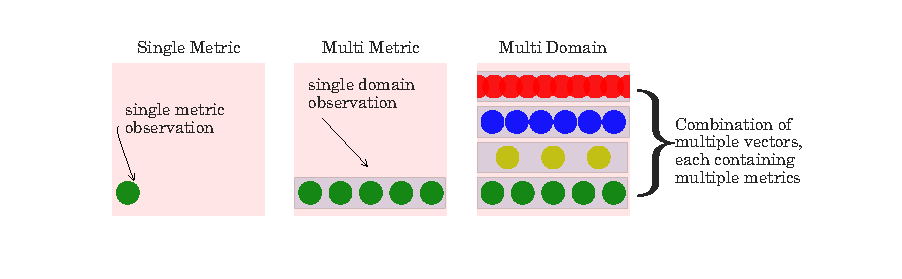
\includegraphics[width=\linewidth]{threat_surface_sum}
	\caption[Multi-Domain Threat Surface]{Multi-Domain Threat Surface}
	\label{fig:threat_surface}
\end{figure}


\subsection{Autonomous Systems Trust and Trust Engineering}

\subsubsection{Autonomous \glspl{manet}}
Autonomy is the capability of an entity to assess its environment and make informed, un-coerced decisions.
In the \gls{manet} context, this sliding scale of capability ranges from basic automated collision avoidance systems while under direct operator control\footnote{For example Automated Driver Assistance Systems entering the consumer vehicle market through the likes of the Tesla P85 and Ford Kuga~\cite{Sawade2016}}, through to self-regulating mission guidance and execution, with limited human interaction\footnote{No such systems have been actively deployed, but this form of collaborative autonomy is the centre of much commercial and academic research\cite{Rajesh2015,Autefage2015,Teke2015}}.
This non-deterministic operation presents significant challenges to security and integrity.
Fundamentally, previously accepted formal verification methodologies for guaranteeing operation are not currently capable of accurately validating the actions and interactions of a fleet or swarm of autonomous nodes in dynamic, noisy environments with imperfect operators~\cite{Teke2015}. 
As such an overlapping combination of ``Secure'' and ``Trusted'' approaches is required throughout the lifecycle and operation of an Autonomous \gls{manet} capability to maintain the integrity of such collaborative systems.

\subsubsection{Trust vs Security vs Integrity}

Early attempts to secure and protect the integrity of \glspl{manet} have relied on various forms of strong-cryptography to protect information being transferred from tampering or malicious inspection.
While such approaches protect the integrity of individual pieces of data, the increased computation, and storage requirements of modern, strong, decentralised cryptographic systems presents a clear avenue for \gls{dos} attacks on \glspl{manet}.
This threat is particularly relevant in resource-constrained networks, where one or more aspects of the environment are limited, be it available power, mobility, data storage, onboard processing, bandwidth, and channel resources such as capacity and delay.
In such networks, where there is a requirement for security and/or integrity monitoring, strong-cryptographic methods present an entirely new opportunity to potential attackers.

One solution to the trade-off between \gls{dos}-protection, and security is the assessment of ``trustworthiness'' of nodes within a local network. 
``Trust'' in this case is an assessment of capability of a node based on previously observed behaviour. \todo{Node/Metric Capability Matrix}
Using this Trust to make simple routing decisions is significantly simpler and faster than strong-cryptographic methods, particularly in multi-hop networks or resource constrained networks~\cite{Cordasco2008}.
With Trust being reliant on the runtime awareness of some behaviour, and cryptography on the pre-establishment of some entropy store and the repeated reinforcement of that numerical security, they represent two very different approaches to system integrity with very different costs/benefits and in practice, some elements of both methodologies will be used in different contexts and applications as those applications dictate.

\subsubsection{Systemic Trust and Trusted Development}
As will be discussed further in \autoref{sec:trust_perspectives}, the ``Trust'' in a system is critical well before a system is activated; the incubation, specification, design, development, production and testing of a system (particularly a system with some \gls{loa} or other non-deterministic operation) is critical to the Trust that an end user can put into that system, and particularly, how much Trust can be exhibited within and between that systems individual components.

\subsubsection{Analytical Trust vs. Game Theoretic/Bio-inspired approaches}
\todo{Analytical Trust vs. Game Theoretic/Bio-inspired approaches}

\subsubsection{Trust Operation Against Capable Attackers}\label{sec:capable_attackers}

In any security situation, the hazards and risks of a systemic vulnerability being identified and exploited by an attacker are tightly coupled to the expectation of capability of that attacker.
Within the context of this work, it is assumed that any attacking agency has the complexity and resources of a nation state.

This is also one of the primary motivators for this particular direction of work; where increasingly complex and subtle evidentiary security measures (passwords, encryption, etc) are applied, with increasing pressures in computation, connectivity, or communication, the assumption that a slightly-higher-technical-investment will protect a system from state-level espionage or infiltration (or the discovery of some technical flaw in the system) is unfounded, with many examples of cryptographic applications being ``disseminated'' through human or technical failings, both internal and external. 

\subsection{Maritime Autonomy}

Given the physical difficulties and requirements of having humans operate underwater (particularly at depth), and the operational limitations of tethered \glspl{rov}, or even untethered remote controlled surface platforms, there has been a great deal of research and commercial interest in the development of autonomous systems, particularly in the defence and petrochemical sectors, where the lives of human operators are most at risk in normal activity~\cite{Pechoucek:2008:DIA:1355335}.

With potential applications ranging from the replacement of human divers in \gls{mcm} activity, to persistent littoral hydrography for environmental flood plain monitoring, many aspects of the proposed efficiencies gained from moving to autonomous agents rely on decentralised, \gls{manet} style collaboration between individual agents, and a level of trust that an operator (or indeed, agents within the system itself) can have in terms of the current activity, readiness, and performance of such autonomous systems~\cite{Wynn2014}.

This ``Trust'', that we understand implicitly in the human space, is particularly difficult to establish and maintain in the underwater environment, and as such, the development of stable, reliable, adaptable trust systems that can operate in this and other challenging environments is a limiting factor on the adoption of generalised distributed autonomous systems in the defence space~\cite{Caseley2009}.

\begin{figure}[h]
	\centering
	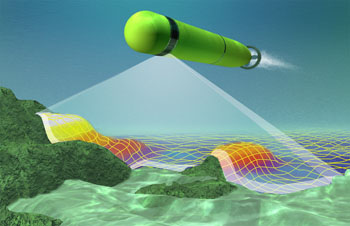
\includegraphics[width=0.8\textwidth]{oceanfloor}
	\caption{An AUV maps the seafloor with sonar \copyright MBARI 2009}
\end{figure}

\pagebreak
\section{Problem Statement}\label{sec:problem}

Within the given context, the primary problem investigated in this work is that of establishing and maintaining trust between a team of mobile autonomous agents (\glspl{auv}) which collaborate over a sparse, noisy, and delayful communications channel (\glspl{uan}) in a distributed fashion to accomplish a specified mission goal (port protection / persistent situational awareness) with the expectation of subversion of one agent within the team by a technically capable actor to exhibit a malicious or selfish behaviour against one or more of the remaining, fairly behaving, agents. 

A secondary problem is that of differentiating between malicious or selfish behaviour and behaviours emerging from damage or misconfiguration of agents (false positive identification).

The proposed solution to these problems is the use of distributed trust assessment across multiple domains of observation (i.e. communications and relative movement), using a weighted grey theoretic grading to synthesise trust observations across metrics and domains to provide a total perspective on the threat surface of agents within a network.
This would constrain the available undetectable misbehaviours of malicious or selfish actors, enforcing ``fair behaviour'' on the network as a whole.
Such filters would be trained against machine learning modelled vectors of ``important metrics'' for particular metrics, ideally reducing the computational complexity of identification and detection. 

This proposal relies on several chained ``problem statement questions'' that require testing.
\begin{enumerate}[label=\textbf{PSQ.\arabic*},ref=\emph{PSQ. \arabic*}]
	\item Given the difference in operation and performance of terrestrial free-space RF vs \gls{uan}, what is an optimal point of data rate and node separation that simultaneously maximises network performance while matching realistic constraints of application? \label{q:rfuan}
	\item How much of existing RF Communications based Trust Management best practice and theory can be carried over to the harsh marine acoustic environment? Indeed, given the long delays and sparse communications, will existing \glspl{tmf} be able to operate at all? Are there any differences in the threats to trust in this new environment? \label{q:uantmf}
	\item Do machine learning and optimisation techniques increase the efficacy of metric weight selection in multi-metric \glspl{tmf} on blind simulations?\label{q:ml}
	\item Can these same or similar approaches to communications Trust be applied to other metric domains, such as the relative position/movement of agents?\label{q:phys}
	\item Can these domains of Trust assessment be combined efficiently while improving detection performance? \label{q:joint}
	\item Is this combined assessment method more effective than domain-only detection? Are there particular classes of misbehaviour that are easy/difficult to identify using these methods? \label{q:perf}
\end{enumerate}

The exploration, experimentation, validation and resolution is best considered visually;
\todo{Block Diagram of Chapter / Experiment Relationships}


\section{Thesis Layout}

\subsubsection{\fullref{ch:trust_background}}
In this chapter, current literature and research on concepts, theory, and applications concerning Trust and Trust Management are explored, specifically leaning towards the applications of Trust within Autonomous \glspl{manet}.

In~\autoref{sec:trust_defs}, the abstract quantity of ``Trust'' is explored.
In~\autoref{sec:trust_autonomy}, Autonomy and ``Trusted Operation'' of autonomous systems is investigated from a system architects and a system operators perspective.
In~\autoref{sec:trust_manets}, current use and applications of Trusted operation of \glspl{manet} is explored, including current \glspl{tmf}.

\subsubsection{\fullref{ch:maritime_background}}
In \autoref{ch:maritime_background}, the maritime context is investigated to support the analysis and modelling of \ref{q:rfuan}, particularly the mechanisms of maritime acoustic communications, as well as the opportunities and challenges of the marine acoustic channel and its modelling (\autoref{sec:marine_comms}).
Additionally, the application scope of \glspl{auv}, littoral and sub-marine operations are explored to provide context to the problems \ref{q:rfuan} and \ref{q:uantmf} (\autoref{sec:marine_ops}).

\subsubsection{\fullref{ch:comms_trust}}
In \autoref{ch:comms_trust}, the need for multi-metric trust assessment in \gls{uan} is demonstrated as an example of a harsh network environment, supporting \ref{q:rfuan}.

The operation of a selection of traditional \gls{manet} \glspl{tmf} is investigated in this environment.
These challenges are characterised and results leveraging a machine learning based optimisation method are presented that demonstrate a multi-metric approach to Trust can greatly enhance the effectiveness of \glspl{tmf} in these environments, supporting \ref{q:uantmf} and \ref{q:ml}.

In~\autoref{sec:initialsystemcharacterization} an experimental configuration for the marine space is established, and the scenarios and results presented in~\citet{Guo11} are reviewed for comparison, which dealt with terrestrial, 802.11 based RF \glspl{manet}.
In~\autoref{sec:trustresultsanddiscussion} findings in trust establishment and malicious behaviour detection are presented, comparing with current single metric \glspl{tmf} (Hermes and \gls{otmf}) and the use of this multi-metric (vector) approach to detecting malicious and selfish behaviour in autonomous marine networks is analysed using \gls{mtfm}.

The contributions of this chapter are the first study on the comparative operation and performance of \glspl{tmf} in \glspl{uan}, and a discussion of metric suitability for \glspl{tmf} in marine environments, informing future metric selection for experimenters and theorists, and identifying both the opportunity and need to generate trust from additional domains, such as the physical domain.
Finally, methodology to assess the usefulness of metrics in discriminating against misbehaviours in such constrained, delay-tolerant networks is demonstrated.

Key parts of this chapter were published as \bibentry{Bolster2015}.

\subsubsection{\fullref{ch:physical_trust}}

Current approaches to operational security have been focused on the establishment of trust/security in the communications domain, and ignore other potential threats to the network exploited through physical movement.
This threat is particularly evident in collaborative autonomous systems where nodes are tasked to accomplish some survey / exploration / observation objective in a distributed fashion, where individual nodes make decisions based on the actions of their ``team''. 
This collaboration opens the opportunity for a physically-misbehaving actor to selfishly conserve it's own resources, or maliciously ``drain'' a given target node.
Current security / trust systems applied to \glspl{manet} are not concerned with the threat of such physical misbehaviours.

This chapter proposes a new approach to trust in resource-constrained networks of autonomous systems based on their physical behaviour, using the motion of nodes within a team to detect and identify malicious or failing operation within a cohort.
This is accomplished by looking at operations within the three dimensions of the underwater space, based on kinematics of industry standard \glspl{auv}.
A series of composite metrics based on physical movement are presented and applied to the detection and discrimination of sample physical misbehaviours.
This approach opens the possibility of bringing information about both the physical and communications behaviours of autonomous \glspl{manet} together to strengthen and expand the application of Trust Management Frameworks in sparse and/or resource constrained environments.

%Key parts of this chapter were published as \bibentry{Bolster2016}.

\subsubsection{\fullref{ch:multi_domain}}

In this chapter a methodology is demonstrated that applies the Grey Relational Grading method used in \gls{mtfm} to assess trust across multiple metrics across multiple domains.
The question of direct-applicability of domain-metrics to inter-domain behaviours (i.e. physical metrics being used to detect communications misbehaviours and visa versa.) is investigated in two stages; first reassessing relative metric significance on a comparative regression directly comparing ``misbehaving'' results and ``Fair'' results across execution runs to identify what metrics are most important in  differentiating behaviours from an abstract perspective. 
This significance is then used to generate targeted weighting vectors to maximally distrust nodes observed exhibiting that behaviour, acting as a selection filter.
From the resultant metric weighting vectors across both basic domains (communications/physical and their full metric union), potential ``Alternate'' domain groupings are selected by inspection.\
By utilising information from multiple domains, it is demonstrated that trust assessment can be more accurate and consistent in identifying misbehaviour than in single-domain assessment.
Further, a methodology for assessing the usefulness of individual metrics in this cross-domain space is demonstrated, allowing for the elimination of redundant metrics, simplifying the runtime assessment process.

{\sloppy \raggedright
Key parts of this chapter are awaiting publication as  \bibentry{Bolster2016a}.
}


\begin{table}\centering
	
	\caption{Summary of Thesis Structure and Contributions}
	\label{tab:thesis_map}
	{\renewcommand{\tabcolsep}{1pt}
		\begin{tabularx}{\textwidth}{p{1.4cm} X X}\toprule
			Chapter 
			& ~~~ Focus 
			& ~~~ Key Outcomes\\ \midrule
			\begin{minipage}[t][][b]{\linewidth}\rot{\parbox{4.5cm}{\fullref{ch:trust_background}}}\end{minipage}
			&\begin{minipage}[t]{\linewidth}
				\begin{tightimize}
					\item Network/Graph theory and Routing
					\item Trust Perspectives, Models and Multi-Party Relationships
					\item Trusted Threats
					\item Autonomy \& Design constraints of Autonomous Systems
					\item Current \glspl{tmf}
				\end{tightimize}
			\end{minipage} 
			&\begin{minipage}[t]{\linewidth}
				\begin{tightimize}
					\item Definition of Trust
					\item Levels \& Constraints of Autonomy
					\item Recognition of Lack Specification \& Validation for Autonomous Systems
					\item Threats to Trust in \glspl{manet}
					\item Need for Trust in Autonomous Systems
				\end{tightimize}
			\end{minipage}\\\midrule
			\begin{minipage}[t][][b]{\linewidth}\rot{\parbox{2.9cm}{\fullref{ch:maritime_background}}}\end{minipage}
			&\begin{minipage}[t]{\linewidth}
				\begin{tightimize}
					\item AUV Operations
					\item Need for Trust in AUV AComms
					\item Marine Acoustics
					\item AComms Modelling 
				\end{tightimize}
			\end{minipage}
			& \begin{minipage}[t]{\linewidth}
				\begin{tightimize} 
					\item Threat Surface
					\item Operational / Kinematic constraints and Scenario selection
					\item Channel Emulation Models
					\item Selection of characteristic channel constraints
				\end{tightimize}
			\end{minipage}\\\midrule
			\begin{minipage}[t][][b]{\linewidth}\rot{\parbox{4.5cm}{\fullref{ch:comms_trust}}}\end{minipage}
			& \begin{minipage}[t]{\linewidth}
				\begin{tightimize} 
					\item Comparative factors between \gls{uan}/\gls{wlan}
					\item Relevant Metric Selection re AComms
					\item Comparison of Single \& Multi Metric \glspl{tmf} in \gls{uan}
					\item \gls{mtfm} weight variation assessment and regression
				\end{tightimize}
			\end{minipage}
			& \begin{minipage}[t]{\linewidth}
				\begin{tightimize} 
					\item Modelled optimal performance range @ $\approx$0.015-0.025pps/100-300m node separations % (\autoref{fig:2d_normed_product})
					\item \gls{mtfm} outperforms single metric \glspl{tmf} for selected misbehaviours % \autoref{fig:otmf_beta_comparison_boxes}
					\item \gls{mtfm} vector weighting further improves performance and tolerance % \autoref{fig:all_mobile_badmouthing}
					\item Long collection times due to sparsity can impact trust assessment relevance
				\end{tightimize}
			\end{minipage}\\\midrule
			
			\begin{minipage}[t][][b]{\linewidth}\rot{\parbox{3.3cm}{\fullref{ch:physical_trust}}}\end{minipage}
			& \begin{minipage}[t]{\linewidth}
				\begin{tightimize} 
					\item Physical Misbehaviours and Metrics
					\item ``Failure'' vs ``Selfish'' vs ``Malice''
					\item \gls{auv} Kinematics
					\item Metric variability in collaborative collision avoidance (flocking)
					\item Metric based classifier
				\end{tightimize}
			\end{minipage}
			& \begin{minipage}[t]{\linewidth}
				\begin{tightimize} 
					\item First physical misbehaviour detection system in \label{uan}
					\item Demonstrate that different misbehaviours impact different physical metrics differently % \autoref{fig:metric_values}
					\item Highly accurate, manually configured, blind behaviour classifier ($\approx$ 0\% FP, $\gtrapprox$ 90 \% TP)
				\end{tightimize}
			\end{minipage}\\\midrule
			\begin{minipage}[t][][b]{\linewidth}\rot{\parbox{4.1cm}{\fullref{ch:multi_domain}}}\end{minipage}
			& \begin{minipage}[t]{\linewidth}
				\begin{tightimize} 
					\item Combination of comms. \& phys. metrics
					\item Random Forest based metric significance correlation to build $H$ weighting vector for \gls{mtfm}
					\item Domain specific behaviour effects across domain space
					\item Relative vector weight measurement across cohort ($\Delta T, \Delta T^-$)
					\item Generation and Appraisal of alternate/targeted ``domains''
				\end{tightimize}
			\end{minipage}
			& \begin{minipage}[t]{\linewidth}
				\begin{tightimize} 
					\item Misbehaviours impact across domains % (not obvious) % \autoref{fig:alternate_domain_diag}
					\item Inherent redundancy (eg \gls{indd}/$P_{RX}$) allows differential behaviours to be detected % \autoref{fig:positive_heat}
					\item Application level selfishness (\gls{sts}) very difficult to automatically detect
					\item Extend \autoref{ch:comms_trust} behaviour based optimisation of \gls{mtfm} to dynamically select most significant metrics
				\end{tightimize}
			\end{minipage}\\
			\bottomrule
		\end{tabularx}
	}
\end{table}





%%%%%%%%%%%%%%%%%%%%%%%%%%%%%%%%%%%%%%%%%%%%%%%%%%%%%%%%%%%%%%%%%%%%%%%%%%%%%%%
